\documentclass[aps,twocolumn,secnumarabic,balancelastpage,amsmath,amssymb,nofootinbib, floatfix]{revtex4-2}

%%%%%%%%%%%%%%%%%%%%%%%%%%%%%%%%%%%%%%%%%%%%%%%%%%%%%%%%%%%%%%%%%%%

\usepackage{float}
\usepackage{graphicx}      % tools for importing graphics
%\usepackage{lgrind}        % convert program code listings to a form 
% includable in a LaTeX document
%\usepackage{xcolor}        % produces boxes or entire pages with 
% colored backgrounds
%\usepackage{longtable}     % helps with long table options
%\usepackage{epsf}          % old package handles encapsulated postscript issues
\usepackage{bm}            % special bold-math package. usge: \bm{mathsymbol}
\usepackage{siunitx}
%\usepackage{asymptote}     % For typesetting of mathematical illustrations
%\usepackage{thumbpdf}
\raggedbottom
\usepackage[colorlinks=true]{hyperref}  % this package should be added after 
% all others.
% usage: \url{http://web.mit.edu/8.13}


%%%%%%%%%%%%%%%%%%%%%%%%%%%%%%%%%%%%%%%%%%%%%%%%%%%%%%%%%%%%%%%%%%%
% And now, begin the document...
%%%%%%%%%%%%%%%%%%%%%%%%%%%%%%%%%%%%%%%%%%%%%%%%%%%%%%%%%%%%%%%%%%%

\begin{document}
	\title{Deriving the Rotation Curve of the Milky Way}
	\author{Octavio Vega}
	\email{ovega84@mit.edu}
	%\homepage{http://web.mit.edu/8.13/} %If you don't have one, just comment out this line.
	\date{\today}
	\affiliation{MIT Department of Physics}
	
	\begin{abstract}
		In this experiment, we observe the dynamics of the Milky Way galaxy, and seek to arrive at a rotation curve for the Milky Way. We compare two primary theoretical models: the classically predicted Keplerian, inverse square-root model as well as a linear, solid body prediction. We collect data on the Doppler shifs of the frequency of the hydrogen 21 cm line using a small radio telescope (SRT) to calculate the radial components of the galactic motion. After analyzing the Doppler shifts at various longitudes in the galactic plane, we compute an experimental rotation curve for the Milky Way. We fit the theoretical models to our data and find that the linear model minimizes the residuals better than the Keplerian model. 
	\end{abstract}
	
	\maketitle
	
	
	%%%%%%%%%%%%%%%%%%%%%%%%%%%%%%%%%%%%%%%%%%%%%%%%%%%%%%%%%%%%%%%%%%%%%%%%
	\section{Background Theory}
	
	\subsection{Gravitation and Rotation}
	
	\begin{figure}
		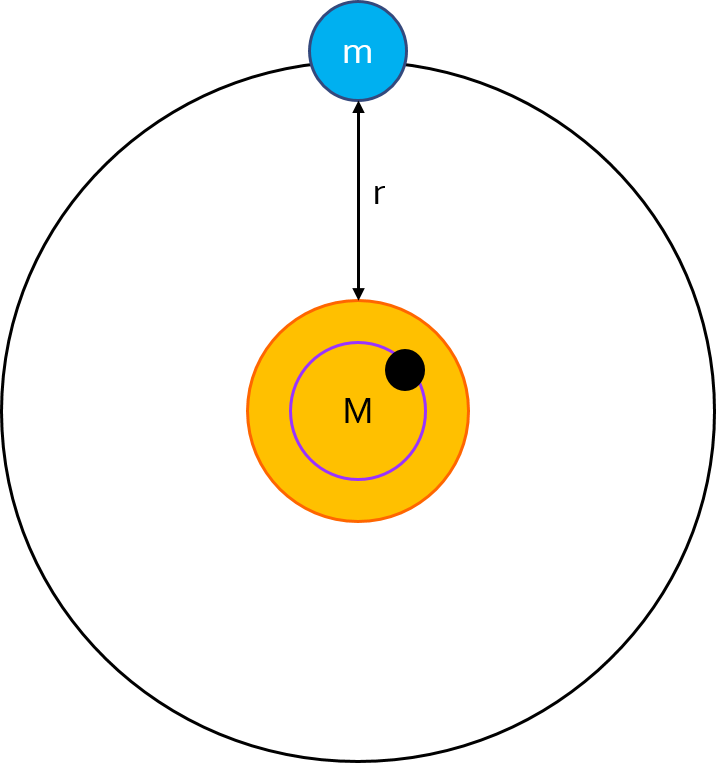
\includegraphics[width=7cm]{orbit_diagram.png}
		\caption{Diagram of orbits of massive objects around a central massive object.}
		\label{fig:orbit}
	\end{figure}
 	Newtonian mechanics provides an important framework with which to make predictions about what form a galactic rotation form will take. Using the diagram shown in~\ref{fig:orbit}, we use classical equations of motion to analyze the behavior of the mass $m$ orbiting the central mass $M$. Using our knowledge of centripetal forces, we can relate the gravitational force of the massive body orbiting the central massive body to its centripetal force via the equation
 	\begin{equation}
 		\frac{mv^{2}}{r}=\sqrt{\frac{GMm}{r^{2}}}
 		\label{eq:centripetal}
 	\end{equation} 
 	where $r$ is the distance from the center of the orbiting body to the center of rotation, and $G$ is Newton's gravitation constant. From equation~\ref{eq:centripetal}, we derive a rotation curve of the form
 	\begin{equation}
 		v(r)=\sqrt{\frac{GM}{r}}
 		\label{eq:keplerian}
 	\end{equation}
 	Hence, we arrive at the Keplerian prediction where the galactic rotational velocity is of the form $v\propto\frac{1}{\sqrt{r}}$. 
 	
 	Alternatively, if we instead consider an imaginary mass rotating within the mass of the central body, we find that we must consider only the fraction of the central mass which is enclosed by the imaginary orbit. Taking the density of the central object to be $\rho$, we find that the mass enclosed is given by 
 	\begin{equation}
 		M(r)=\rho V(r)=\rho \frac{4}{3}\pi r^{3}
 	\end{equation}  
 	Hence, using the centripetal force relation~\ref{eq:centripetal}, we find this rotation curve to be
 	\begin{equation}
 		v(r)=\sqrt{\frac{4\rho G \pi r^{2}}{3}}
 		\label{eq:solidbody}
 	\end{equation}
 	Therefore the solid-body prediction for the rotation curve has the form $v(r)\propto r$, which is a linear relationship. 
	\begin{figure}
		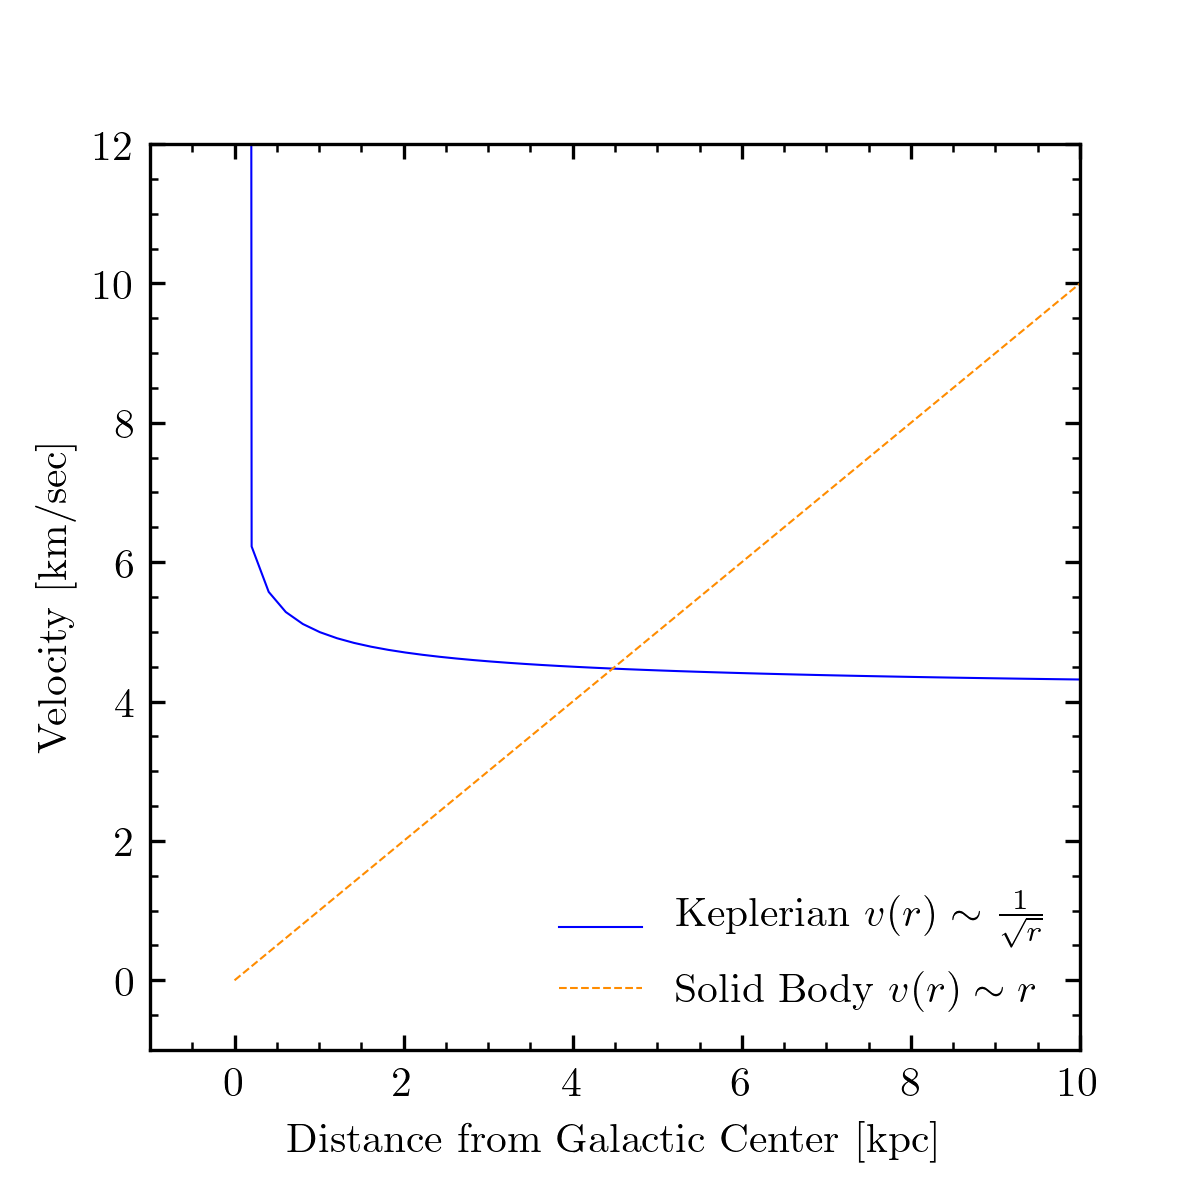
\includegraphics[width=9cm]{theo_rot_curves.png}
		\caption{Theoretical rotation curves of the Milky Way as functions of the distance from the galactic center.}
		\label{fig:model}
	\end{figure}
	
	Figure~\ref{fig:model} displays the comparison between the Keplerian and solid-body models of rotation curves. We predict that our experimental rotation curve may exhibit behavior similar to either of the models individually, or perhaps some linear combination of them. 
	
	\subsection{The Hydrogen Spin-Flip}
	
	The theoretical components of our ability to use the apparatus to measure frequency spectra is a key consequence of the quantum mechanical behavior of hydrogen atoms. The interstellar medium is comprised of an abundance of atomic hydrogen, whose atoms exhibit a convenient quantum mechanical phenomenon which we leverage for the purposes of this experiment. 
	
	It is well known that due to the presence of stars and interstellar dust, visible light is heavily obfuscated and suffers absorption from these objects. However, wavelengths of light outside of the visible spectrum, specifically at $\lambda_{0}=21$ cm, can suffer much less absorption. 
	
	Neutral hydrogen atoms contain a nucleus and a single electron. The discretization of angular momentum states in quantum mechanics allows the spin states of the proton and the electron to be either parallel or anti-parallel. The nature of the wavefunctions describing these states is such that the anti-parallel configuration exists at a lower energy than the parallel spin configuration. When the hydrogen atom transitions from the latter state to the former, it emits energy which, according to $E=hf_{0}$, has a frequency of $f_{0}=1420.4$ MHz, equivalent to a wavelength $\lambda_{0}=21$ cm. This is the hydrogen spin-flip line.
	
	\subsection{Geometry of the Milky Way and Galactic Rotation Curves}
	In the final motivational section of this paper, we discuss the geometric relationships between various kinematic quantities of interest in the Milky Way. We use each of these quantities to arrive at a rotation curve $v(r)$ of the galaxy.
	
	\begin{figure}
		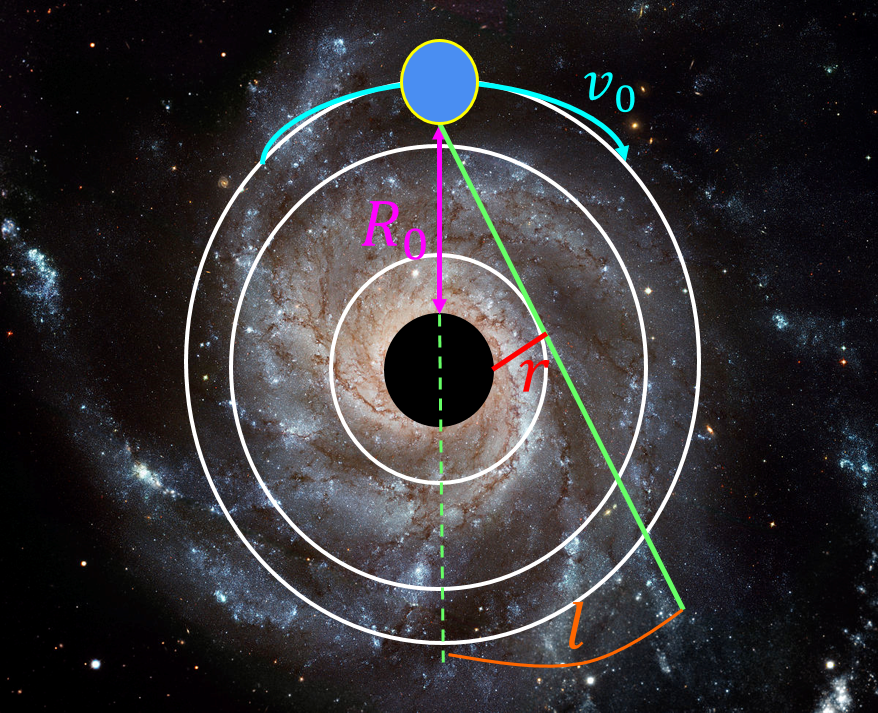
\includegraphics[width=7cm]{galactic_geometry.png}
		\caption{Diagram of the geometric relationships between kinematic quantities in the Milky Way.}
		\label{fig:geometry}
	\end{figure}
	
	The independent variable of our rotation curve will be the radii $r$, i.e. the distance from the galactic objects being observed to the center of the galaxy. We take the distance from our solar system to the galaxy to be $R_{0}=$, compute the radii from the galactic longitudes $l$ at which we point our telescope via the relation
	\begin{equation}
		r=R_{\odot}\sin(\frac{l\pi}{180^{\circ}})
		\label{eq:radii}
	\end{equation}
	We also consider the Doppler-shifted frequences of the 21 cm line, from which we can derive the speed of the observed object, i.e. the source $s$, given by 
	\begin{equation}
		v_{s}=\frac{f_{0}-f_{\mathrm{red}}}{f_{0}}c
		\label{eq:doppler}
	\end{equation}
	where $f_{0}1420.4$MHz is the frequency of the 21 cm line, $f_{\mathrm{red}}$ is the maximally red-shifted 21 cm line frequency, and $c$ is the speed of light. 
	From this, we can compute the maximum radial velocity of the source along the telescope's line of sight, which is given by 
	\begin{equation}
		v_{\mathrm{max}}=v_{s}-v_{\mathrm{lsr}}
		\label{eq:vmax}
	\end{equation}
	where we subtract the velocity of our local standard of rest $v_{\mathrm{lsr}}$ to remove any rotation we have with respect to the sun.
	
	Finally, we compute the velocity curve by combining equation~\ref{eq:vmax} with the rotational velocity $v_{\odot}$ of the solar system:
	\begin{equation}
		v(r)=v_{\mathrm{max}}+v_{\odot}\sin(\frac{l\pi}{180^{\circ}})
	\end{equation}

	
	%%%%%%%%%%%%%%%%%%%%%%%%%%%%%%%%%%%%%%%%%%%%%%%%%%%%%%%%%%%%%%%%%%%%%%%%
	\section{Experimental Procedure}

	\subsection{The SRT Circuit}
		\begin{figure}[H]
		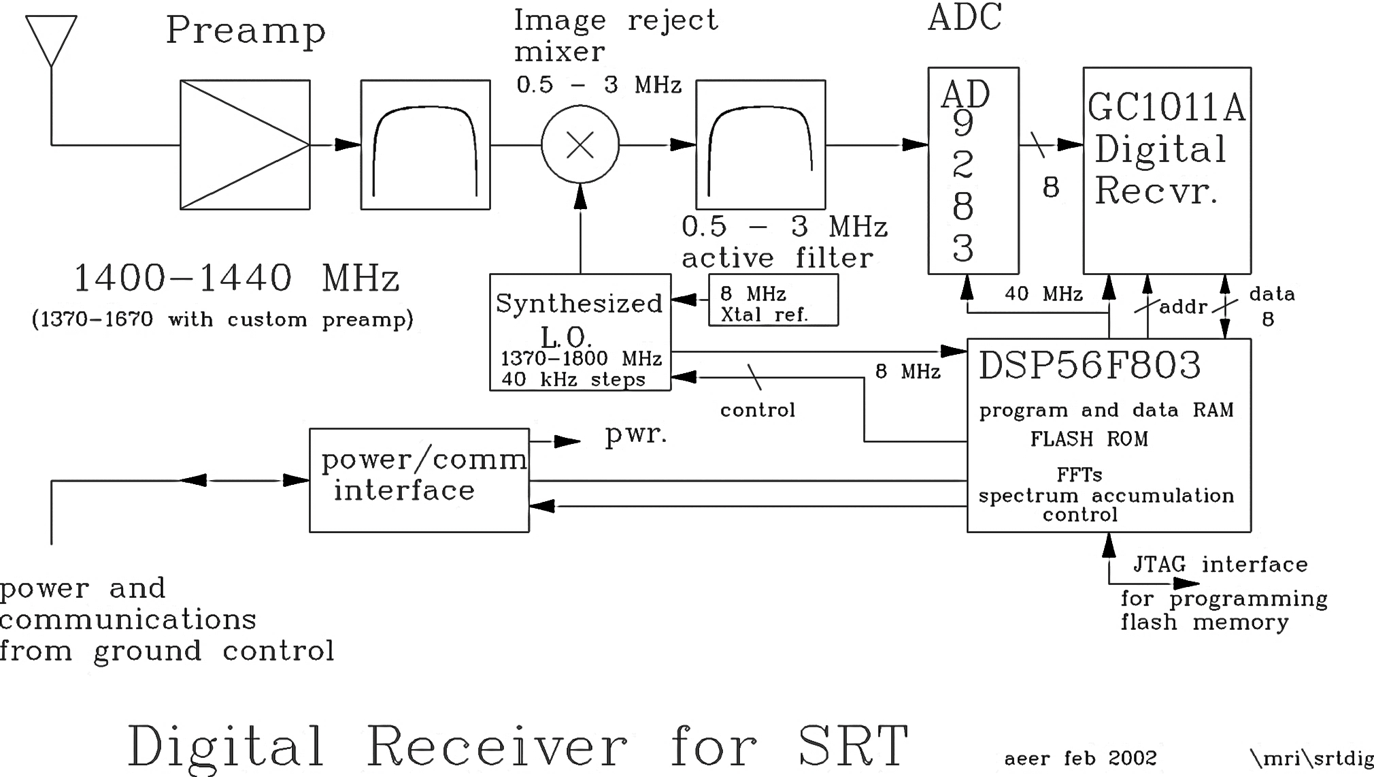
\includegraphics[width=9cm]{circuit_diagram.png}
		\caption{Circuit diagram for the SRT digital receiver. Taken from the Junior Lab 21cm Radio Astrophysics \cite{labmanual}}.
		\label{fig:circuit}
	\end{figure}
	One of the most important components of the SRT circuit is the image reject mixer, which modulates the incoming signal by multiplying it by another sinusoid. By the laws of trigonometry, the resulting signal is of the form $\cos(\omega_{1}t)\cos(\omega_{0}t)=\frac{1}{2}\cos((\omega_{0}+\omega_1)t)+\frac{1}{2}\cos((\omega_{1}-\omega_{0})t)$.
	
	The band pass filter in the SRT circuit then attenuates the first signal in the sum, leaving only the signal with frequency equal to the difference $\omega_{1}-\omega_{0}$. This is crucial as we will study the Doppler shifted frequencies while gathering data. 

	
	\subsection{Measurement Procedure}
	To gather data, we always begin by pointing the telescope at an empty region of the sky, and calibrating the telescope via the SRT interface to remove background noise. We then scan over eight separate galactic longitudes between $20^{\circ}$ and $90^{\circ}$ in increments of $10^{\circ}$, allowing the SRT to perform 20 scans at each galactic coordinate and average the results to arrive at our temperature spectra for each coordinate. 
	
	To perform these scans, we utilize command files that dictate instructions to the telescope, including where to point and how many scans to perform. We feed our command files into the SRT interface, allowing the data to be taken automatically. Note that the calibration step is performed at the start of each data taking session, so we always list a calibration of the telescope as the first step in our command files.  
	

	%%%%%%%%%%%%%%%%%%%%%%%%%%%%%%%%%%%%%%%%%%%%%%%%%%%%%%%%%%%%%%%
	\section{Data and Error Analysis}
	
	
	In this section I present raw data collected, as well as our reduced data followed by a discussion on the relevant errors and their sources. 
	
	\subsection{Frequency Spectra}
	At each galactic coordinate, we receive a temperature (intensity) spectrum in 148 frequency bins of width 0.0078125 MHz. In~\ref{fig:rawspec70} I display the raw temperature spectrum at the galactic longitude $70^{\circ}$.
	 
. 	\begin{figure}[h]
		\centering
		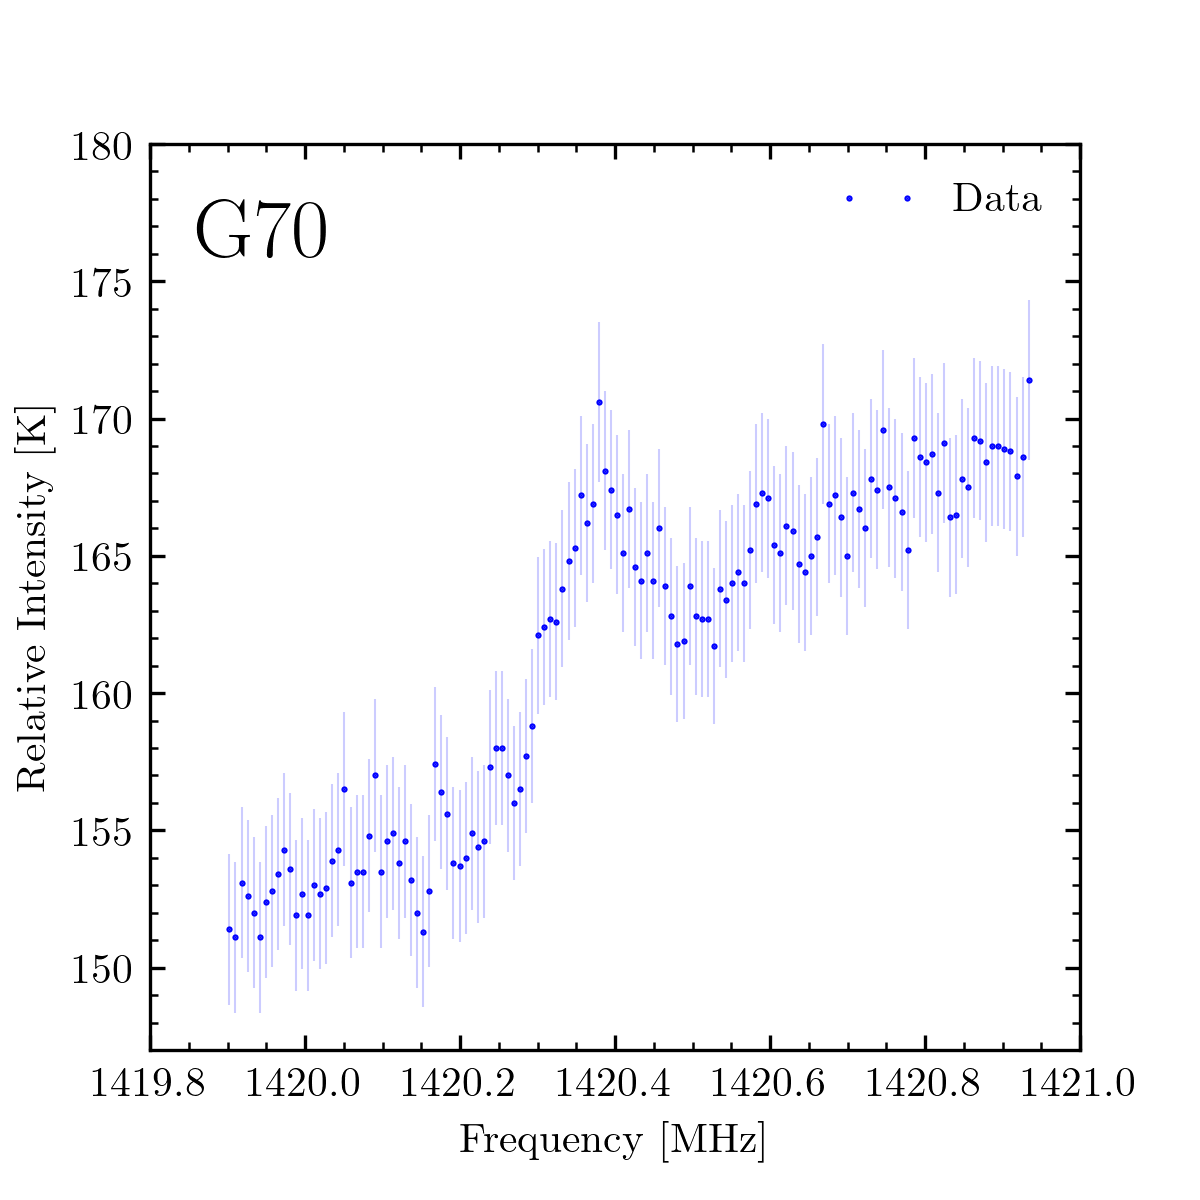
\includegraphics[width=9cm]{spec_linraw_70.png}
		\caption{The raw temperature spectrum in frequency bins for the galactic longitude $l=70^{\circ}$.}
		\label{fig:rawspec70}
	\end{figure}
	
	Upon receiving these raw spectra, our next step is to fit the data to a linear background model $y=ax+b$, where $a$ and $b$ are fit parameters.~\ref{fig:linspec70} displays the best fit linear background model to the raw data.
	
	\begin{figure}[h]
		\centering
		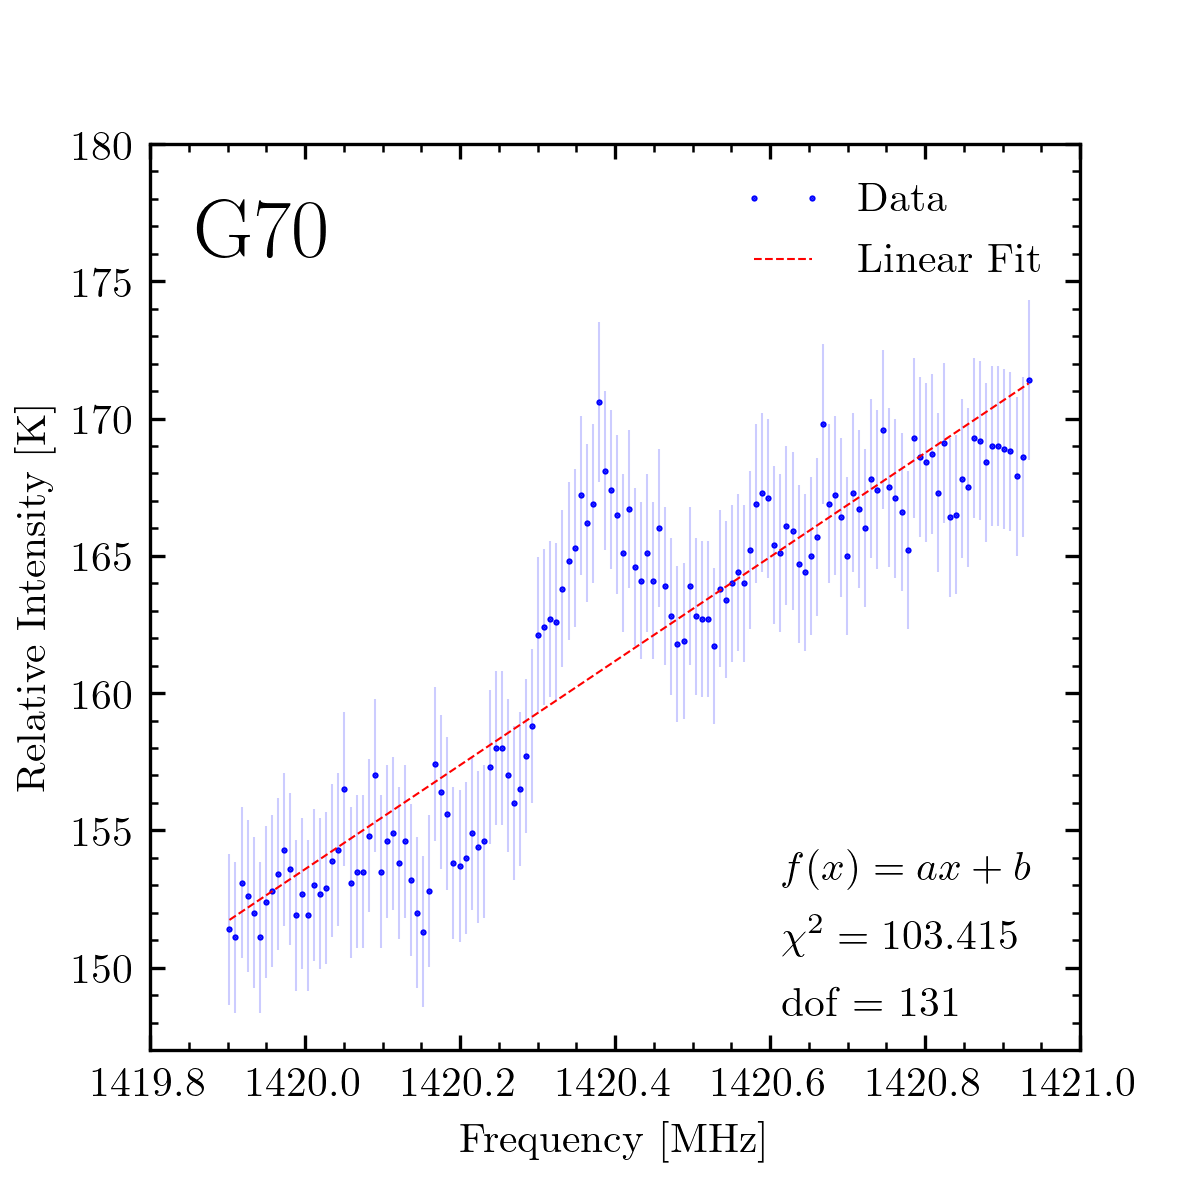
\includegraphics[width=9cm]{spec_linfit_70.png}
		\caption{The temperature spectrum for $l=70^{\circ}$ with best fit linear background model superimposed in red, along with resulting fit parameters $a$ and $b$ and the $\chi^{2}$ value for the fit.}
		\label{fig:linspec70}
	\end{figure}
	
	Finally, in order to determine the maximally red-shifted frequencies, our last step is to remove the background from the raw data by subtracting the linear models from each of our raw temperature spectra. From this, we fit a new functional to the resulting spectra, which takes the form
	\begin{equation}
		f(x)=\sum_{i=1}^{4}a_{i}e^{\frac{-(x-\mu_{i})}{2\sigma_{i}^{2}}} + b
	\end{equation} 
	
	To find the maximually red-shifted frequency $f_{\mathrm{red}}$, we take the least mean fit parameter $\mu_{i}=f_{\mathrm{red}}$, as this would correspond to the greatest shift $f_{0}-f_{\mathrm{red}}$.
	
	~\ref{fig:gaussspec70} gives an example for $l=70^{\circ}$ of this background-removed spectrum with such a functional fit. 
	
	\begin{figure}[h]
		\centering
		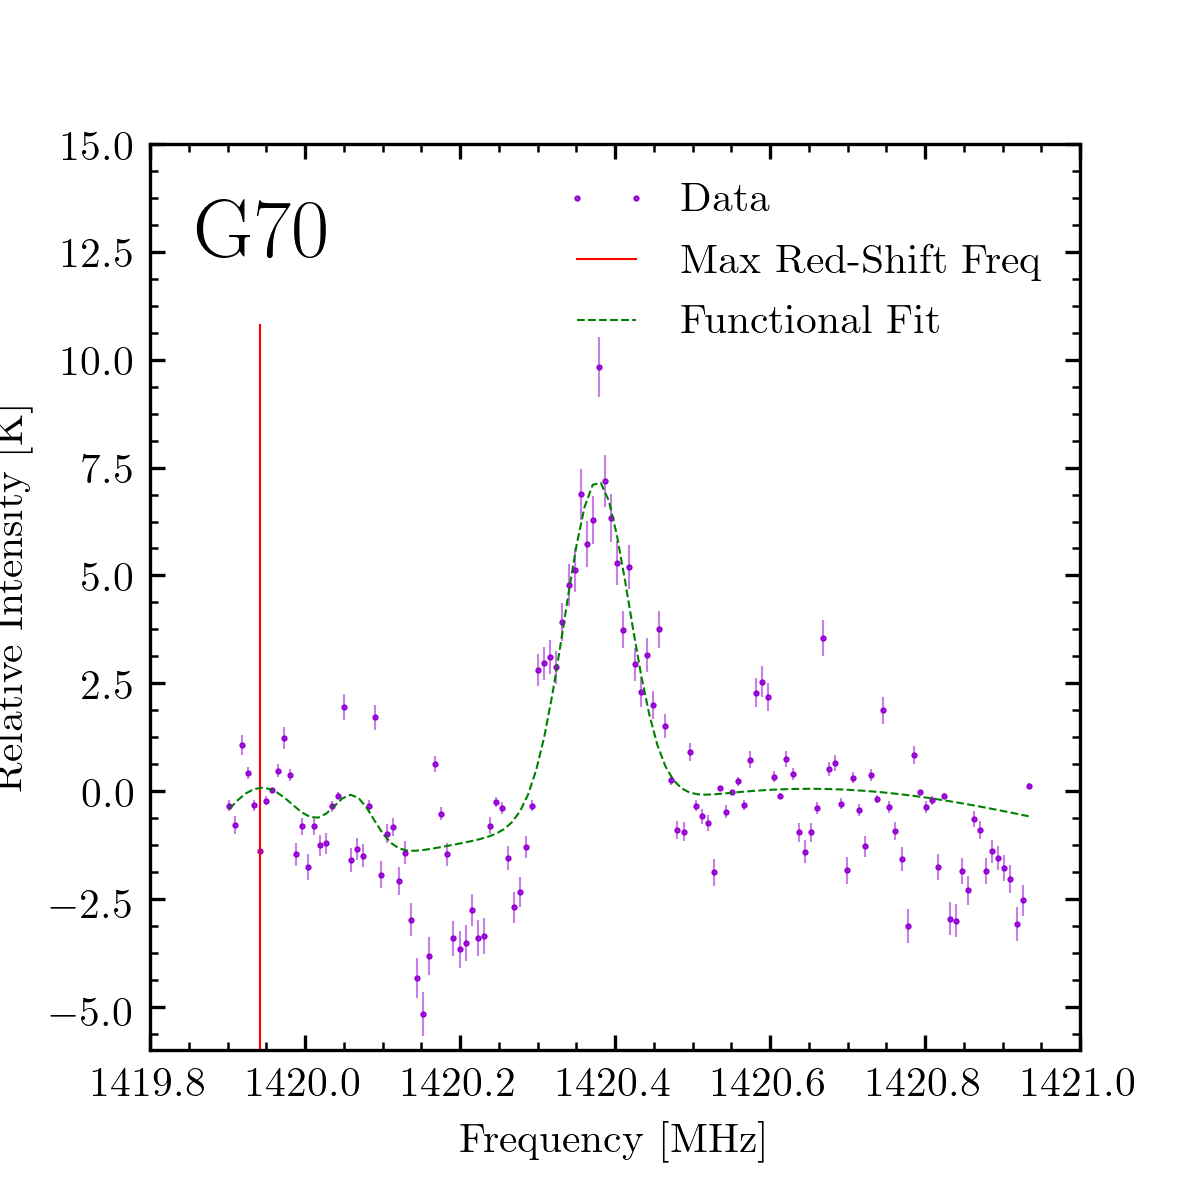
\includegraphics[width=9cm]{spec70_gauss_fit.png}
		\caption{The background-removed temperature spectrum for $l=70^{\circ}$, as well as the best fit curve of the sum of four gaussian functions and constant offset.}
		\label{fig:gausspec70}
	\end{figure}
	
	\subsection{Dark Matter and Observed Rotation Curves}
	We recall that our two predicted models for the Milky Way rotation curves are given by the relationships $v(r)\propto \frac{1}{\sqrt{r}}$ and $v(r)\propto r$ for the Keplerian and solid-body models, respectively. 
	
	Due to the observation of physicists of the presence of unobserved mass as speculated by rotation curves not exhibiting a $\frac{1}{\sqrt{r}}$ fall-off but rather a somewhat linear relationship, we now call the solid-body model the 'dark matter' prediction.
	
	Using our equations from section I.3, we are able to use our data to calculate a velocity curve for the milky way.
	
	In testing the goodness of fit of the rotation curve modes to our rotation curve data, I do not fit the functions to the entire dataset. Instead, I only consider the velocity data points at a radius greater than 6 kpc, because I am mainly concerned with how the curve falls off outside of the central bulge of the Milky Way where the greatest mass is concentrated. I fit the models to the velocity data external to the Milky Way bulge, as seen in figure~\ref{fig:rotfit}.
	\begin{figure}
		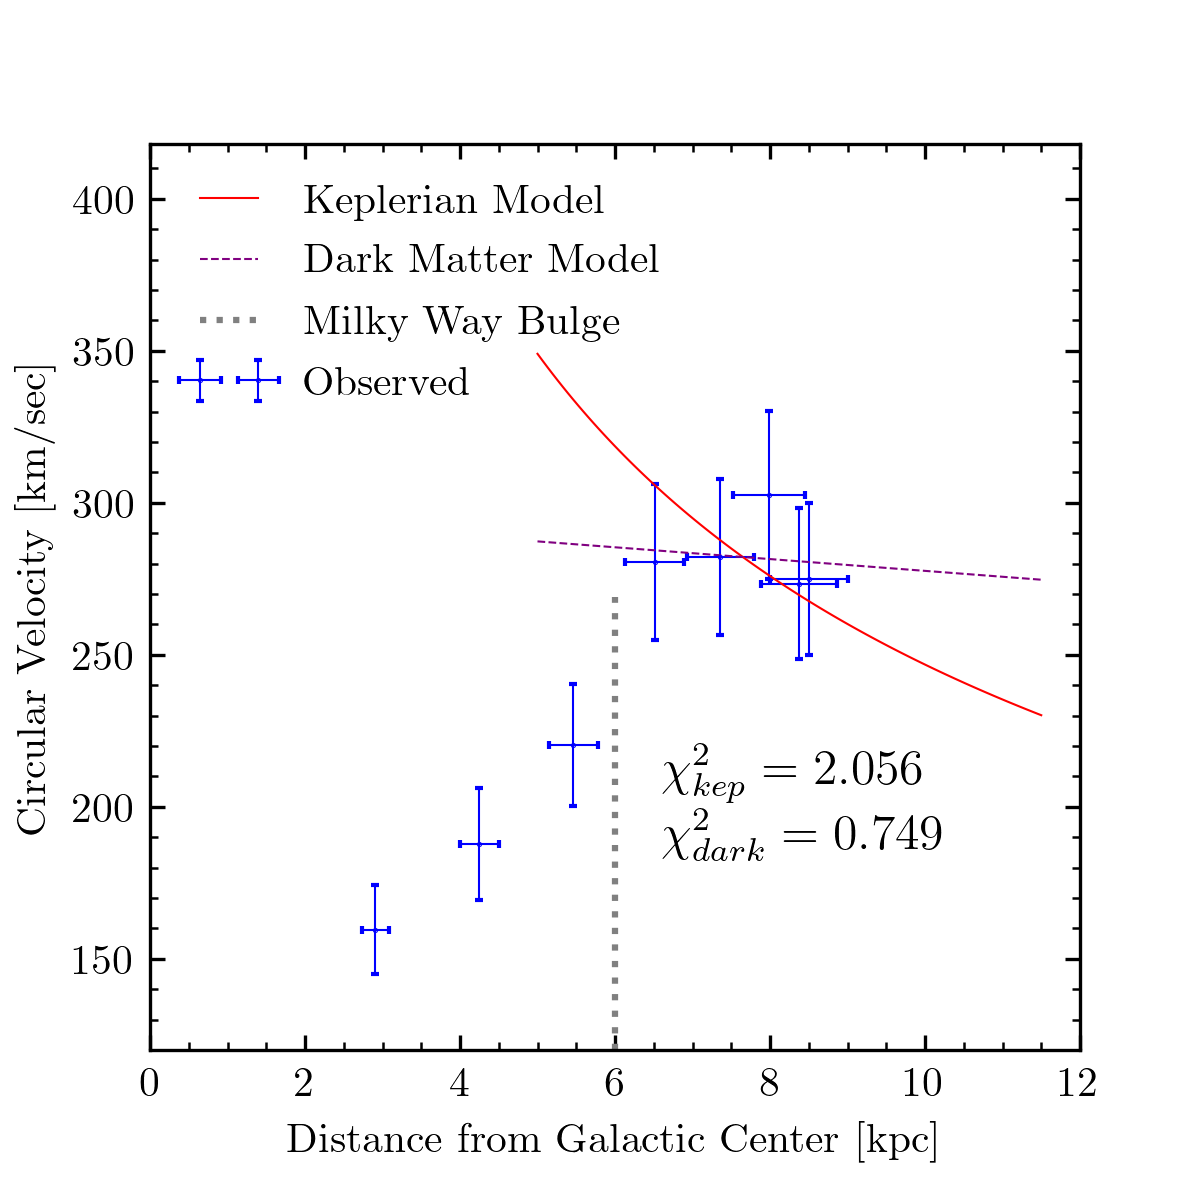
\includegraphics[width=9cm]{rot_curve_fit.png}
		\caption{The velocity data, superimposed on which are the functions of best fit, each corresponding to one of the two initial models for the rotation curve. The $\chi^{2}$ statistic for the fits is also displayed in the plot.}
		\label{fig:rotfit}
	\end{figure}


	After fitting the two functional forms to the data, we find that $\chi^{2}_{\mathrm{dark}}<\chi^{2}_{\mathrm{kep}}$. Hence, the linear model, which is more predictive of potential dark matter, fits to our experimental velocity curve much better than the initial Keplerian prediction for $v(r)$.
	
	\subsection{Error Estimation and Discussion}
	I attribute contributors to statistical uncertainties throughout this experiment mainly to the scarcity of data points.
	\begin{itemize}
		\item much fewer independent galactic longitudes $l$ scanned than desired
		\item no longitudes $l<20^{\circ}$ were scanned
		\item only one session of data gathering per each longitude was performed
	\end{itemize}
	
	I attribute the sources of the systematic uncertainty to a number of factors as well:
	\begin{itemize}
		\item some of the low-longitude scans were performed at such a time that they were beginning to exit the telescope's field of view, meaning that the signal strengths were much weaker for these coordinates
		\item our fit function to find the maximally red-shifted frequencies is not precisely motivated by a theory, but motivated by an inspection of the peak structure of the background-removed spectra
		\item two of the days of data taking occurred during heavy rain and cloud cover, possibly interfering with the SRT
	\end{itemize}  
	
	
	%%%%%%%%%%%%%%%%%%%%%%%%%%%%%%%%%%%%%%%%%%%%%%%%%%%%%%%%%%%%%%
	\section{Conclusions}
	By using the MIT Junior Lab SRT to measure the 21cm hydrogen line frequency, we observed the maximum red-shift of frequencies emitted from the neutral hydrogen cloud in the atmosphere. With these data, synthesized with our geometric analysis of the Milky Way, we were able to obtain an experimental rotation curve for the galaxy and compare it to known models. we ultimately found a better fit for the dark-matter prediction than for the classical Keplerian prediction.
	
	Whether there is dark matter in the universe is a question for further experimentation. Nonetheless, our finding that our data heavily favors the dark-matter model is an amazing result. With more careful attention to the galactic longitude scans and greater amounts of data over time, we hope to replicate these results and use them in the future to derive the spiral-arm structure of the Milky Way.
	
	
	%%%%%%%%%%%%%%%%%%%%%%%%%%%%%%%%%%%%%%%%%%%%%%%%%%%%%%%%%%%%%%%%%%%%%%%
	\begin{acknowledgments} The author is very grateful to Luke Gianni for serving as his lab partner throughout this experiment. The author is also very thankful for the constructive feedback offered by Professor Fakhri. The author would additionally like to thank Hanzhen Lin for their useful discussions on various related topics. 
	\end{acknowledgments}
	
	%%%%%%%%%%%%%%%%%%%%%%%%%%%%%%%%%%%%%%%%%%%%%%%%%%%%%%%%%%%%%%%%%%%%%%%%% 
	
	\bibliography{paper2}
	
\end{document}
